\section{Work plan}

To reach the goals of this project, the project is divided into six phases. Each phase leads to a milestone at the end of the phase and has also a time buffer of one week. An overview of the work plan can be seen as a Gantt chart in Figure \ref{fig:workplan}. Each phase is now explained in detail in the following Sections.

\subsection{Data Acquisition}
\label{phase:data_aqui}
For the first phase, a workload of six weeks is scheduled. It is also divided into three subphases. Firstly, a phase to understand and analyze the equipment for data recording. In the pre-studies, the microphone and speaker were already used but for the SLAM approach we need sound recordings in combination with position data. For that, several options are given by the Lab which have to be compared and understood. One example which could be used for measuring position data is the HTC Vive.

During this phase, the next phase can start where data is acquired for later analysis. This data could also have position data but that's not necessary. This data is used to compare different approaches for continuous functions based on the RIR. It also should show later whether the RIR with moving speaker will behave similarly to the approach from Dokmanic \cite{dokmanic_roomrecslam_2016} as described in Section \ref{sec:acoustic_slam}.

After the analysis data is collected and all equipment is understood, the test and validation data can be gathered. This data should be used later to test and validate the implemented SLAM approach. So it should be a combination of sent output, recorded input, and position data for every timestep $t$.

The milestone of this phase will be to gather analysis, test, and validation data. If this phase will unexpectedly take much longer so the whole project will be in danger, at least the RIR approach explained in Chapter \ref{chap:pre_studies} can be applied to the data to show whether the RIR for moving speakers behave continuously. 

\subsection{Data Analysis}
\label{phase:data_analysis}
After the data acquisition phase, the data has to be analyzed in this phase to derive a continuous function suitable for SLAM and approximable with Gaussian Processes in real-time. For this, a workload of seven weeks is scheduled. This phase is also divided into two phases. The first phase to analyze the data and find suitable continuous functions. In the second one these continuous functions found in the phase before are compared to find the most suitable for our case.

The milestone in this phase will be to find out the most promising continuous functions derived from the acoustic signal usable for SLAM approaches. If the project needed too much time until this phase, several approaches for continuous functions suitable for SLAM could be published which shows that acoustic SLAM is probably suitable for completely unprepared environments.

\subsection{Gaussian Process Optimization}
This phase will be a short phase with a workload of one week. In this phase, the Gaussian processes will be optimized for the different continuous functions given by the phase before. During optimization, the most suitable kernel has to be found and the best fitting parameter set up for this kernel has to be optimized. So the milestone will be a set of optimal Gaussian processes for the given functions. If no time after this phase is left for further work, a paper of the functions suitable for SLAM with some plots of the continuous function in space could be published.

\subsection{Implementation of Test Environment and SLAM Approach}
A workload of five weeks is scheduled for this phase. This phase is divided into three phases. During the first phase a test environment is implemented to simulate a virtual robot with the data given by the phase described in Section \ref{phase:data_aqui}. This test environment is also used for later evaluation purposes. The next phase is to plot a map of the continuous functions to finally see if it's suitable for SLAM and if there are any errors or other issues within the data or with the derived functions. In the end, a SLAM approach will be implemented which is also the milestone of this phase. As in the phase before, if no time is left the derived functions and plots showing the continuous functions suitable for SLAM can be published. 

\subsection{Test and Validation}
The test and validation phase is scheduled with a workload of three weeks and is divided into three subphases. First testing the SLAM approach given by the phase before in the test environment. After that, the SLAM approach should be tested on real data with a robot platform. At the end, the results should be compared to other approaches especially to the one from Dokmanic \cite{dokmanic_roomrecslam_2016} described in Section \ref{sec:acoustic_slam}. The milestone of this phase will be the validation of this approach and the comparison to others. If the time is getting short, the test on real data could be canceled and the SLAM approach will only be tested in the virtual environment on the data given by the first phase described in Section \ref{phase:data_analysis}. 

\subsection{Paper}
In the end, all knowledge of the project has to be gathered and written down into a paper. For that, a workload of three weeks is scheduled. It seems a little bit short but every phase should produce a short document with the milestone. Also, each phase has a buffer of one week. So if every phase before will work as planned, there will be six weeks buffer left for this phase. The milestone of this phase will be the paper. 

\begin{figure}[hp]
	\centering
	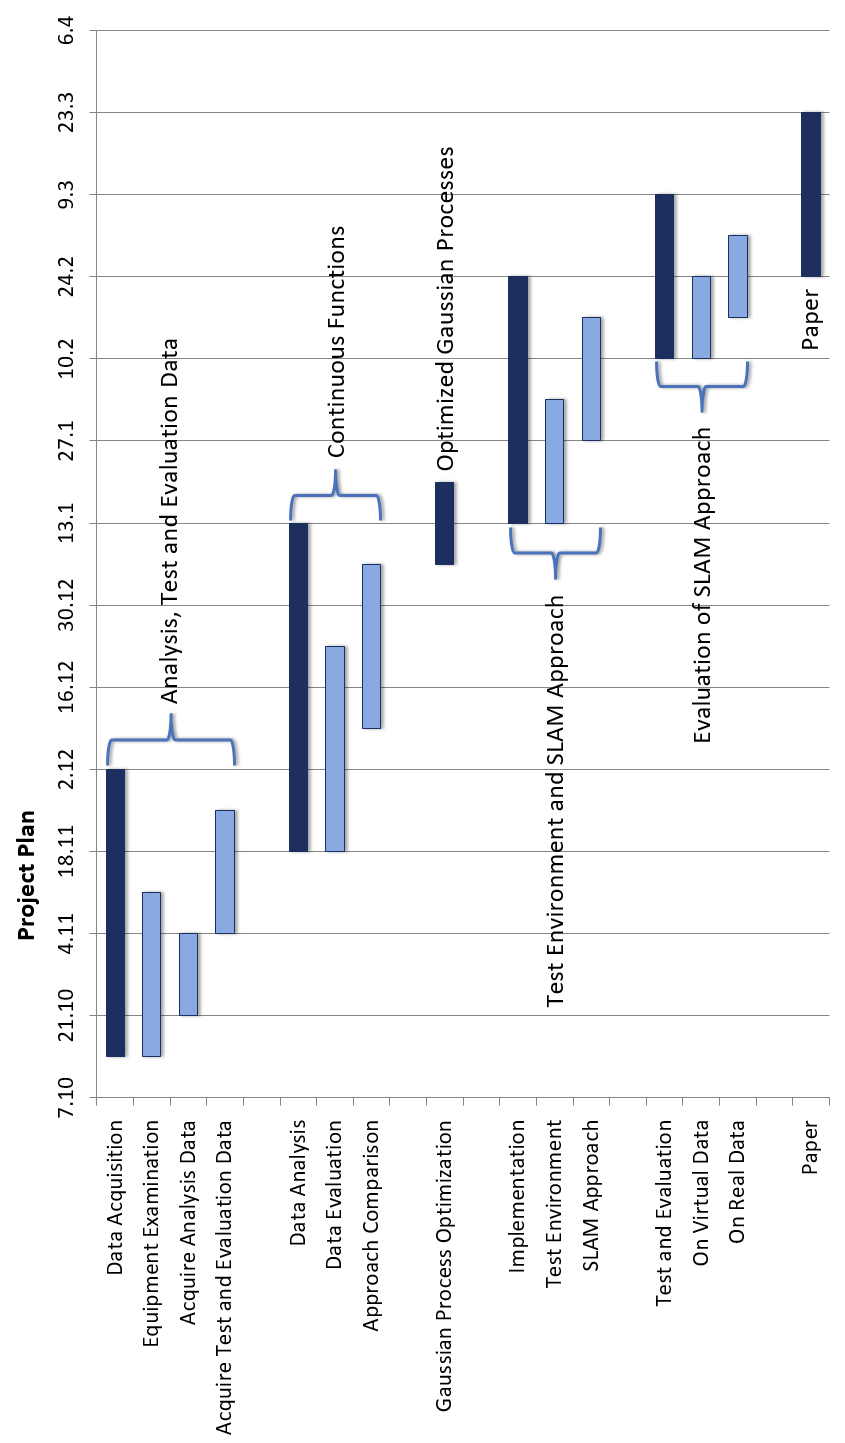
\includegraphics[width=\textwidth]{images/projectplan.png}
	\caption{
		Gantt chart to illustrate the project plan.
	}
	\label{fig:workplan}
\end{figure}
\newpage